\chapter{Flow Charts}
\label{Chapter8}

\section{Initial/MainWindow Flow Charts}
\begin{figure}[H]
	\centering
	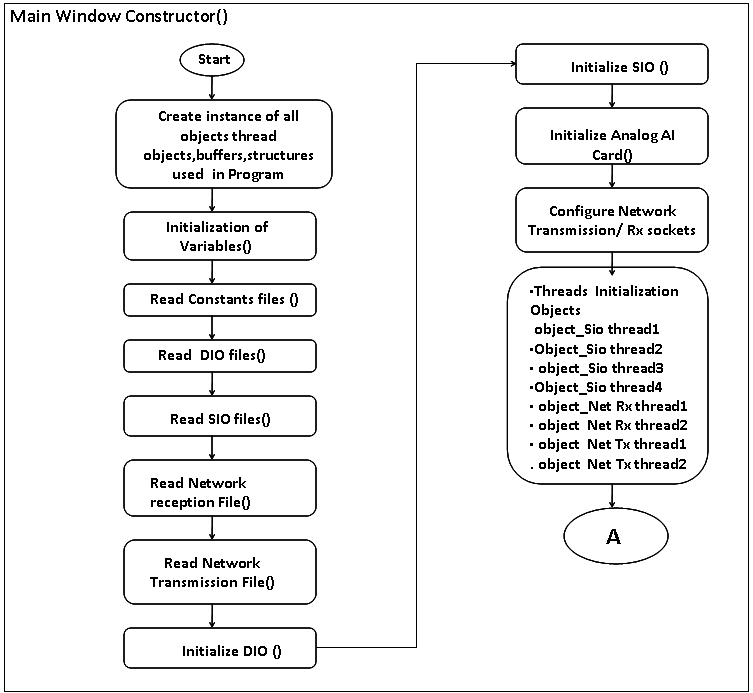
\includegraphics[width=\linewidth]{./FlowCharts/PngFlowCharts/Main1.png}
	%\caption{Five Chain Configuration of Telecommand}
	%\label{FIG:FiveChConfig}
\end{figure}
\begin{figure}[H]
	\centering
	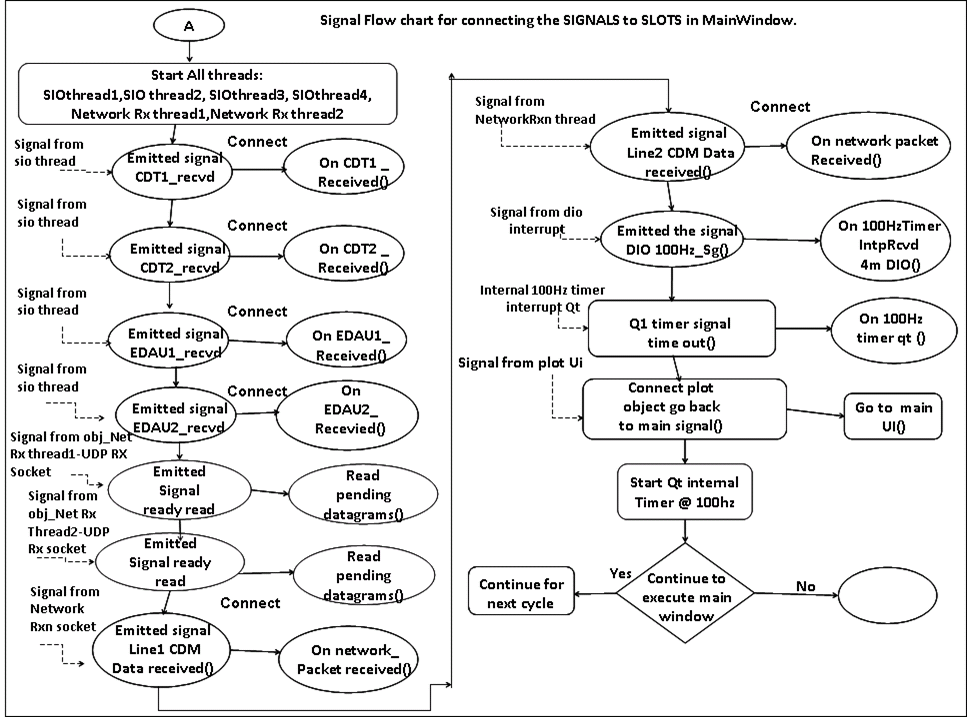
\includegraphics[width=\linewidth]{./FlowCharts/PngFlowCharts/Main2.png}
	%\caption{Five Chain Configuration of Telecommand}
	%\label{FIG:FiveChConfig}
\end{figure}
\section{Flow charts of slots in mainWindow}
\subsection{CDT Slot Flow Charts in mainWindow}

\begin{figure}[H]
	\centering
	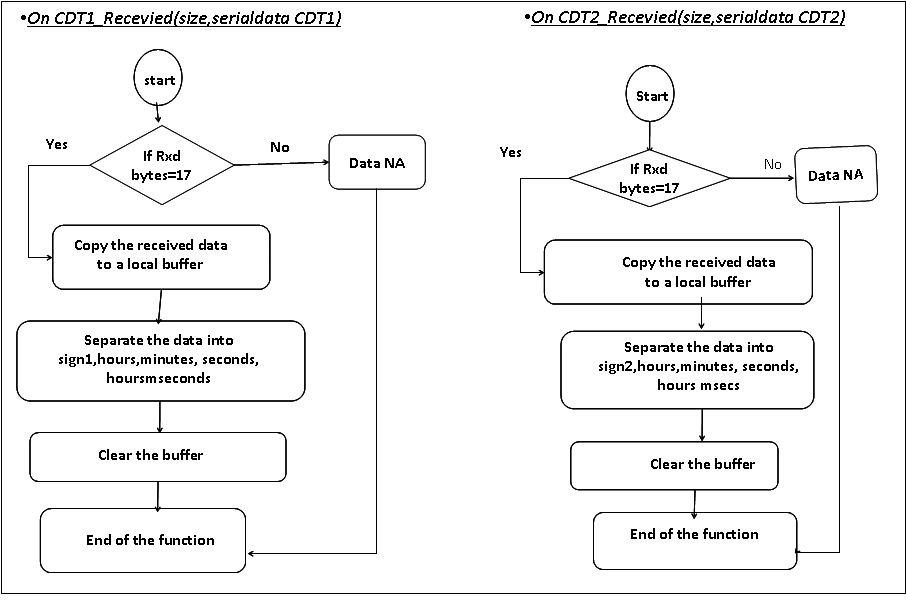
\includegraphics[width=\linewidth]{./FlowCharts/PngFlowCharts/SLOT_CDT12.png}
	%\caption{Five Chain Configuration of Telecommand}
	%\label{FIG:FiveChConfig}
\end{figure}
\subsection{EDAU Slot Flow Charts in mainWindow}

\begin{figure}[H]
	\centering
	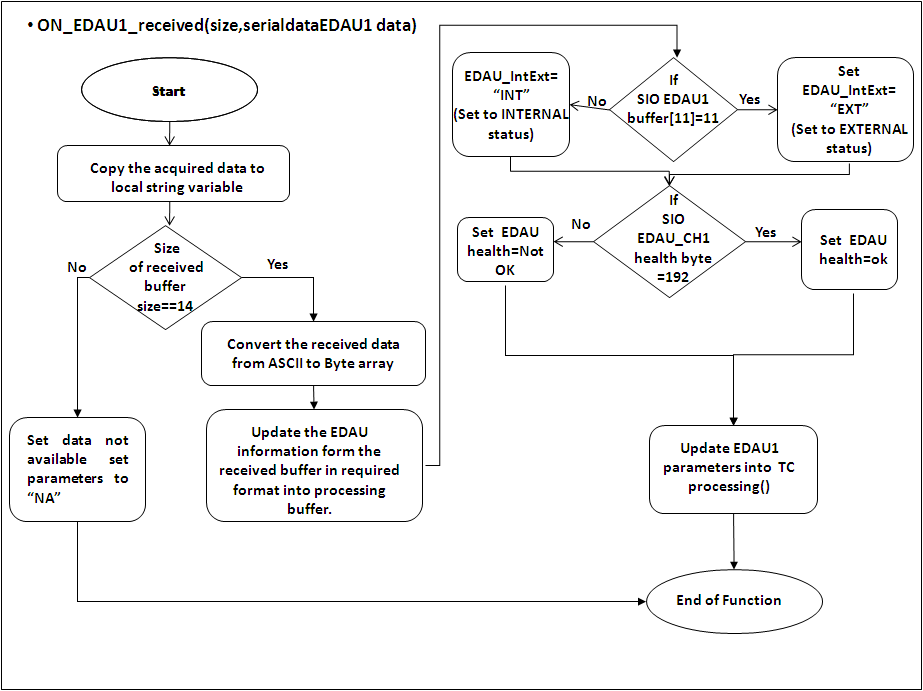
\includegraphics[width=\linewidth]{./FlowCharts/PngFlowCharts/SLOT_EDAU1.png}
	%\caption{Five Chain Configuration of Telecommand}
	%\label{FIG:FiveChConfig}
\end{figure}
\begin{figure}[H]
	\centering
	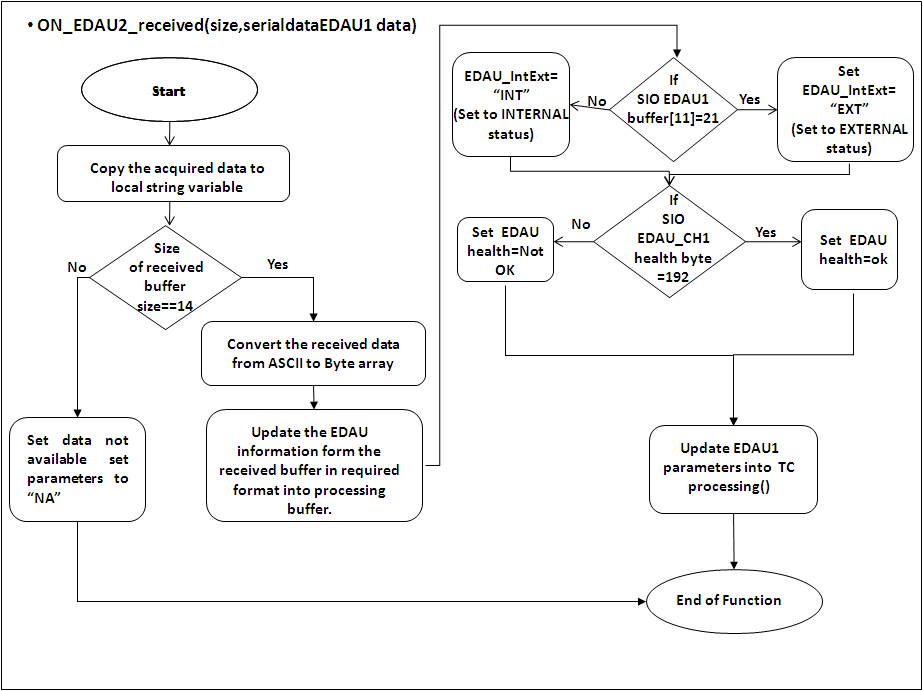
\includegraphics[width=\linewidth]{./FlowCharts/PngFlowCharts/SLOT_EDAU2.png}
	%\caption{Five Chain Configuration of Telecommand}
	%\label{FIG:FiveChConfig}
\end{figure}

\subsection{CDM Slot Charts in mainWindow}

\begin{figure}[H]
	\centering
	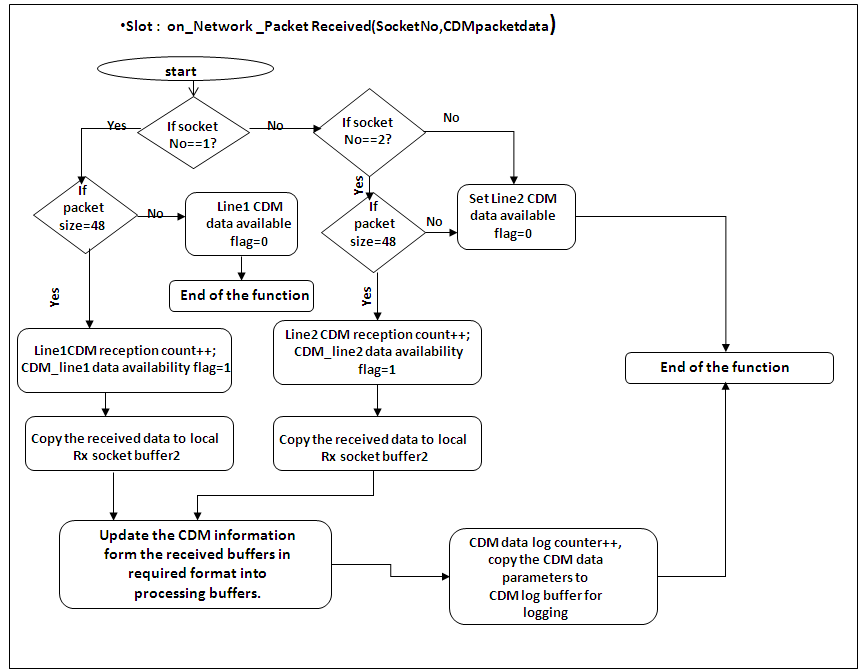
\includegraphics[width=\linewidth]{./FlowCharts/PngFlowCharts/SLOT_CDM.png}
	%\caption{Five Chain Configuration of Telecommand}
	%\label{FIG:FiveChConfig}
\end{figure}

\subsection{100Hz Interrupt received slot in mainWindow}
\begin{figure}[H]
	\centering
	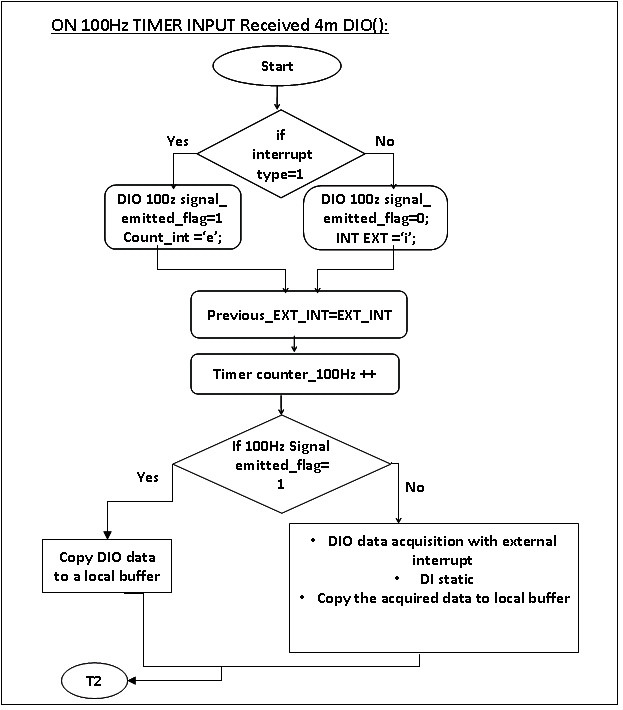
\includegraphics[width=\linewidth]{./FlowCharts/PngFlowCharts/SLOT_100Hz1.png} 
	%\caption{Five Chain Configuration of Telecommand}
	%\label{FIG:FiveChConfig}
\end{figure}
\begin{figure}[H]
	\centering
	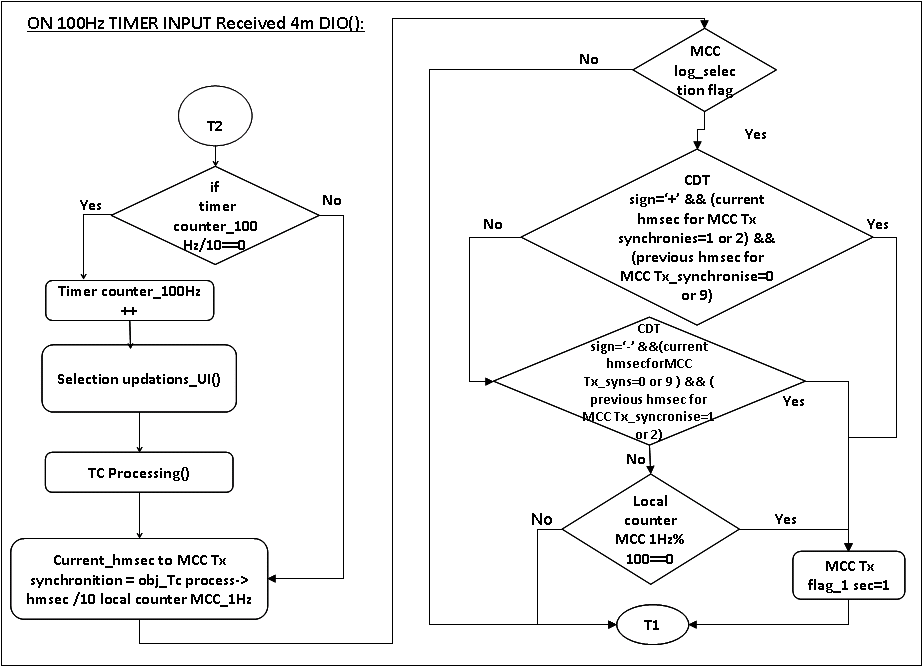
\includegraphics[width=\linewidth]{./FlowCharts/PngFlowCharts/SLOT_100Hz11.png} 
	%\caption{Five Chain Configuration of Telecommand}
	%\label{FIG:FiveChConfig}
\end{figure}
\begin{figure}[H]
	\centering
	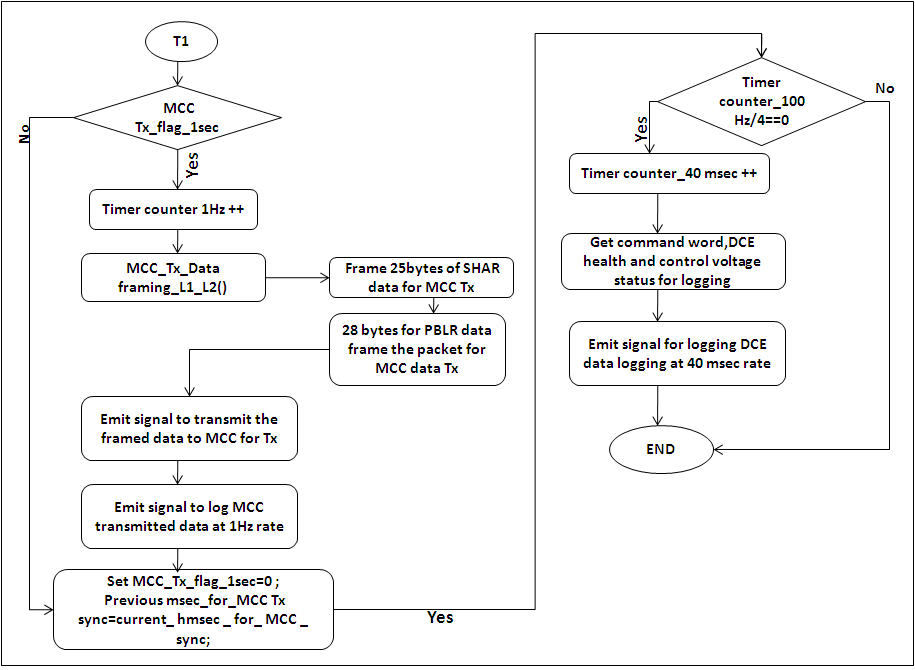
\includegraphics[width=\linewidth]{./FlowCharts/PngFlowCharts/SLOT_100Hz2.png} 
	%\caption{Five Chain Configuration of Telecommand}
	%\label{FIG:FiveChConfig}
\end{figure}

\subsection{TcProcess Flow charts: in mainWindow}

\begin{figure}[H]
	\centering
	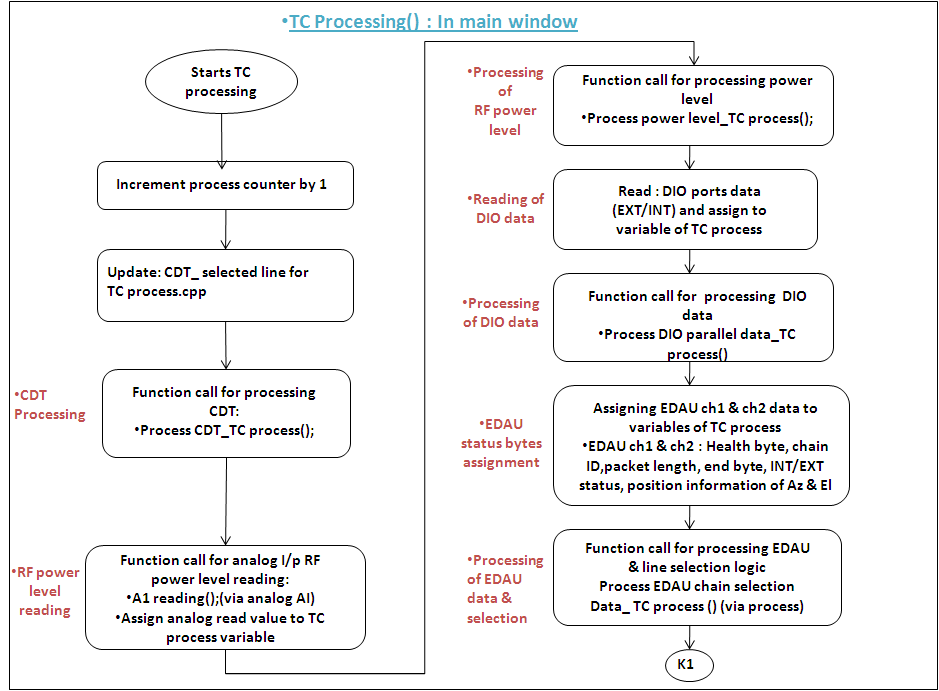
\includegraphics[width=\linewidth]{./FlowCharts/PngFlowCharts/TCP1.png}
	%\caption{Five Chain Configuration of Telecommand}
	%\label{FIG:FiveChConfig}
\end{figure}

\begin{figure}[H]
	\centering
	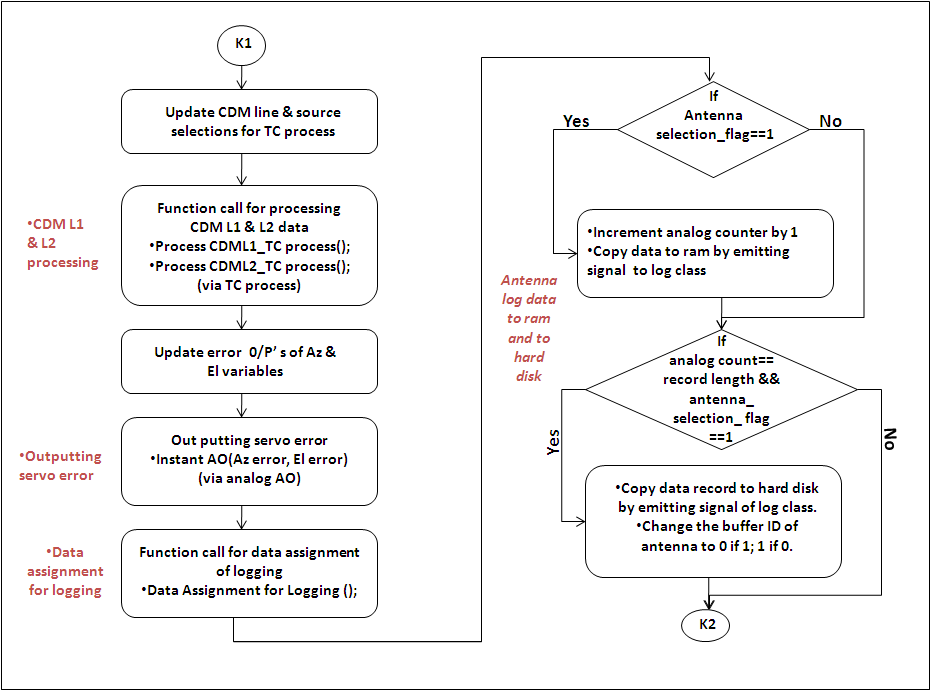
\includegraphics[width=\linewidth]{./FlowCharts/PngFlowCharts/TCP2.png}
	%\caption{Five Chain Configuration of Telecommand}
	%\label{FIG:FiveChConfig}
\end{figure}

\begin{figure}[H]
	\centering
	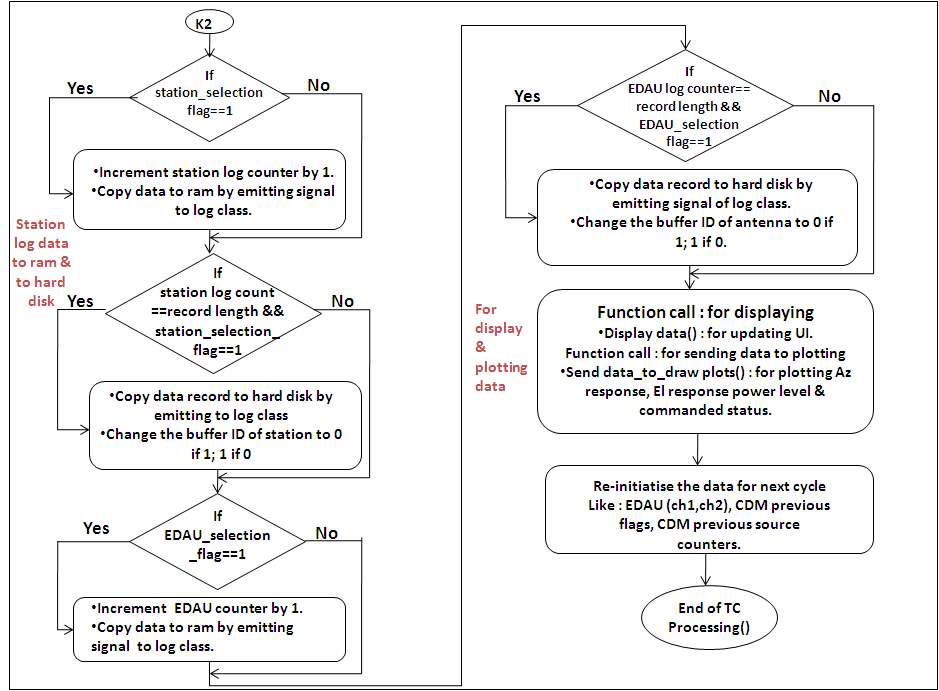
\includegraphics[width=\linewidth]{./FlowCharts/PngFlowCharts/TCP3.png}
	%\caption{Five Chain Configuration of Telecommand}
	%\label{FIG:FiveChConfig}
\end{figure}
\subsection{Data assignment for logging: in mainWindow}
\begin{figure}[H]
	\centering
	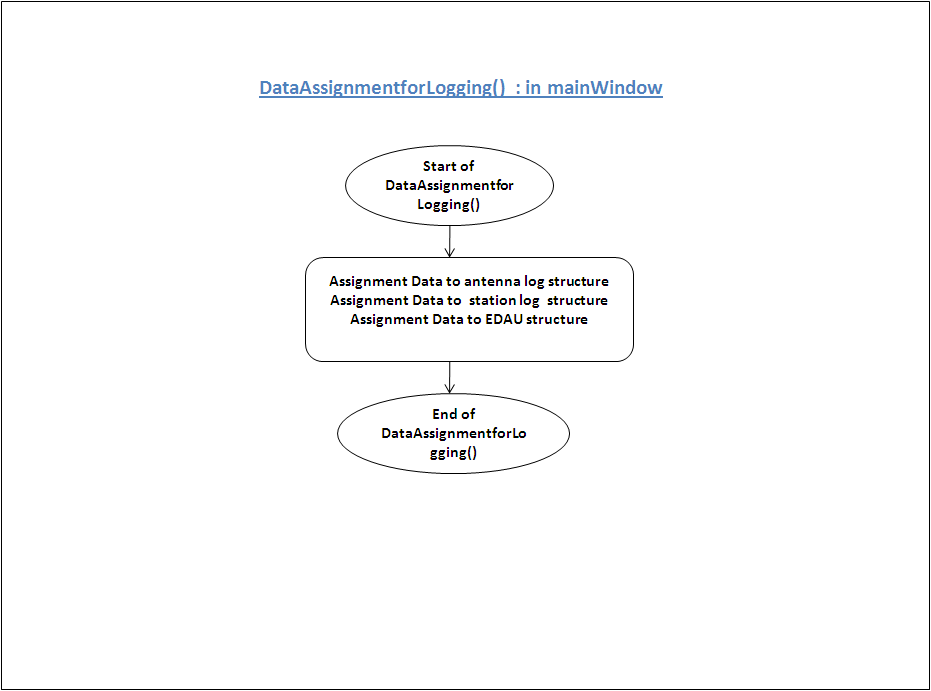
\includegraphics[width=\linewidth]{./FlowCharts/PngFlowCharts/TCP11.png}
	%\caption{Five Chain Configuration of Telecommand}
	%\label{FIG:FiveChConfig}
\end{figure}
\section{TC process flow charts : tcprocess class}
\subsection{CDT Processing}
\begin{figure}[H]
	\centering
	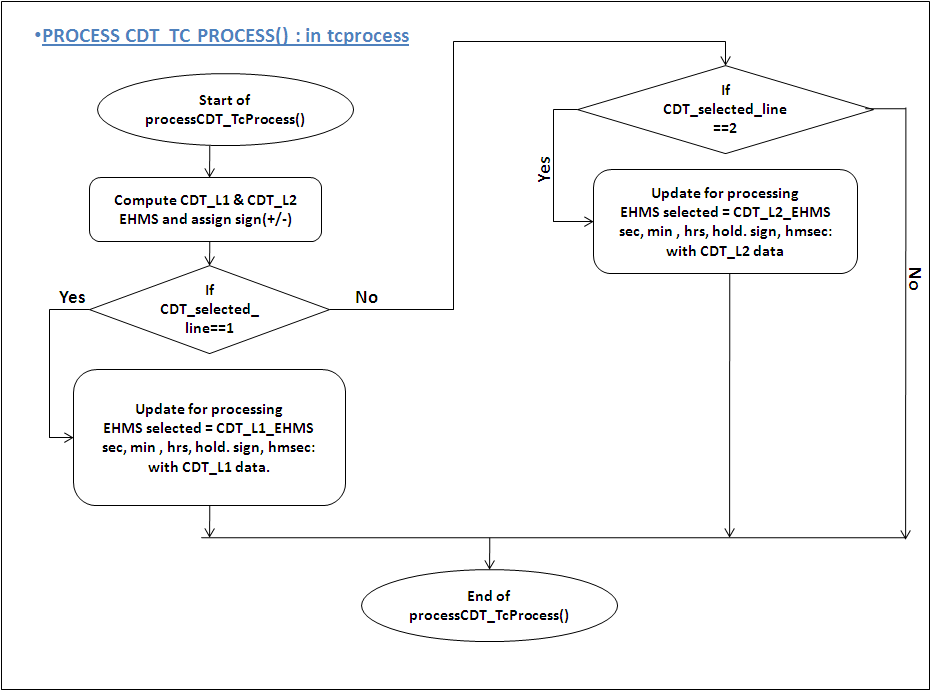
\includegraphics[width=\linewidth]{./FlowCharts/PngFlowCharts/TCP4.png}
	%\caption{Five Chain Configuration of Telecommand}
	%\label{FIG:FiveChConfig}
\end{figure}
\subsection{RF power level processing}
\begin{figure}[H]
	\centering
	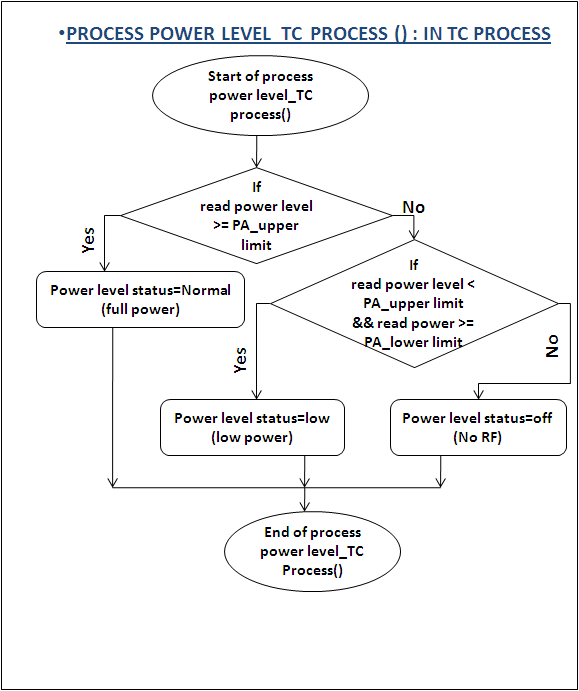
\includegraphics[width=\linewidth]{./FlowCharts/PngFlowCharts/TC_PA.png}
	%\caption{Five Chain Configuration of Telecommand}
	%\label{FIG:FiveChConfig}
\end{figure}

\subsection{DIO parallel data processing}
\begin{figure}[H]
	\centering
	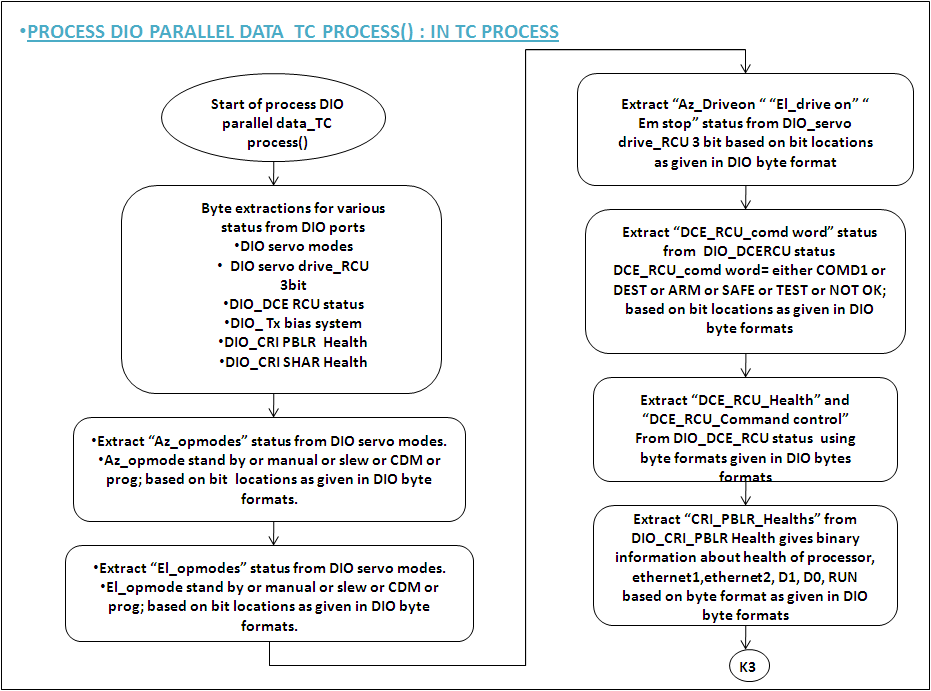
\includegraphics[width=\linewidth]{./FlowCharts/PngFlowCharts/TCP6.png}
	%\caption{Five Chain Configuration of Telecommand}
	%\label{FIG:FiveChConfig}
\end{figure}

\begin{figure}[H]
	\centering
	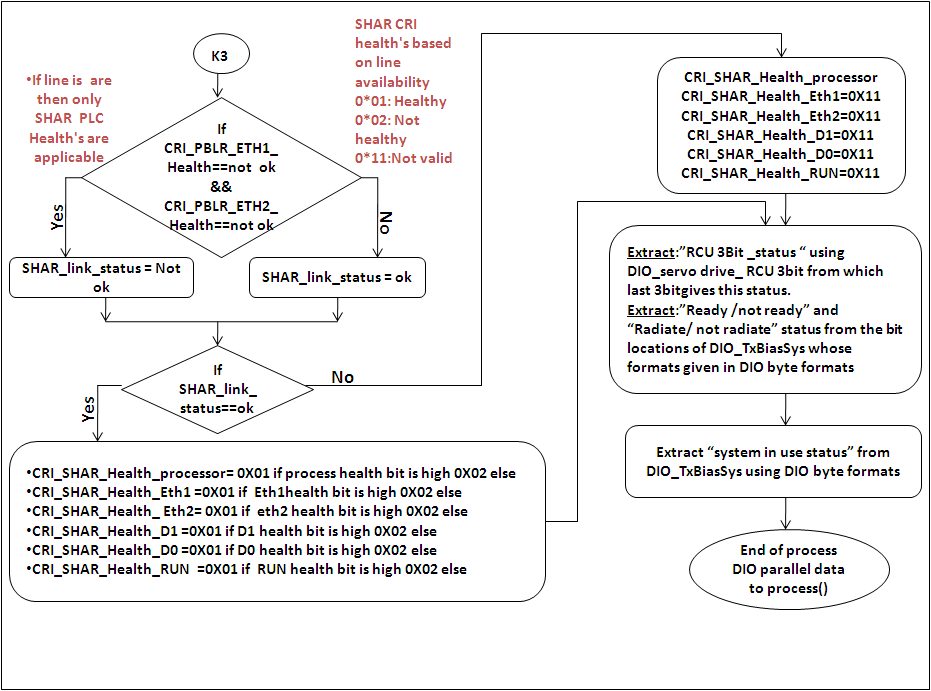
\includegraphics[width=\linewidth]{./FlowCharts/PngFlowCharts/TCP7.png}
	%\caption{Five Chain Configuration of Telecommand}
	%\label{FIG:FiveChConfig}
\end{figure}

\subsection{CDM data processing}
\begin{figure}[H]
	\centering
	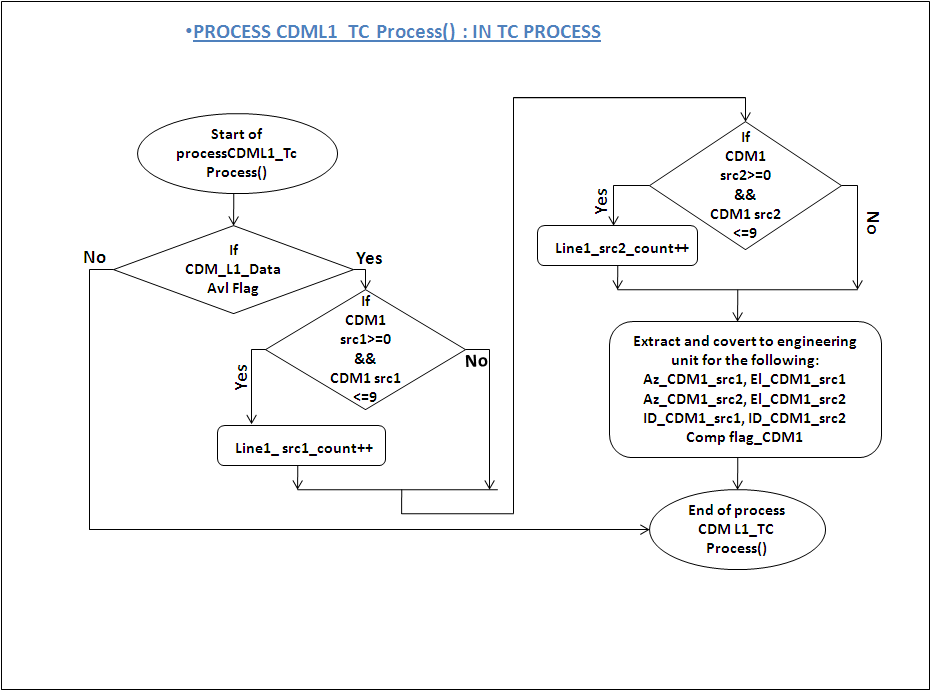
\includegraphics[width=\linewidth]{./FlowCharts/PngFlowCharts/TCP8.png}
	%\caption{Five Chain Configuration of Telecommand}
	%\label{FIG:FiveChConfig}
\end{figure}

\begin{figure}[H]
	\centering
	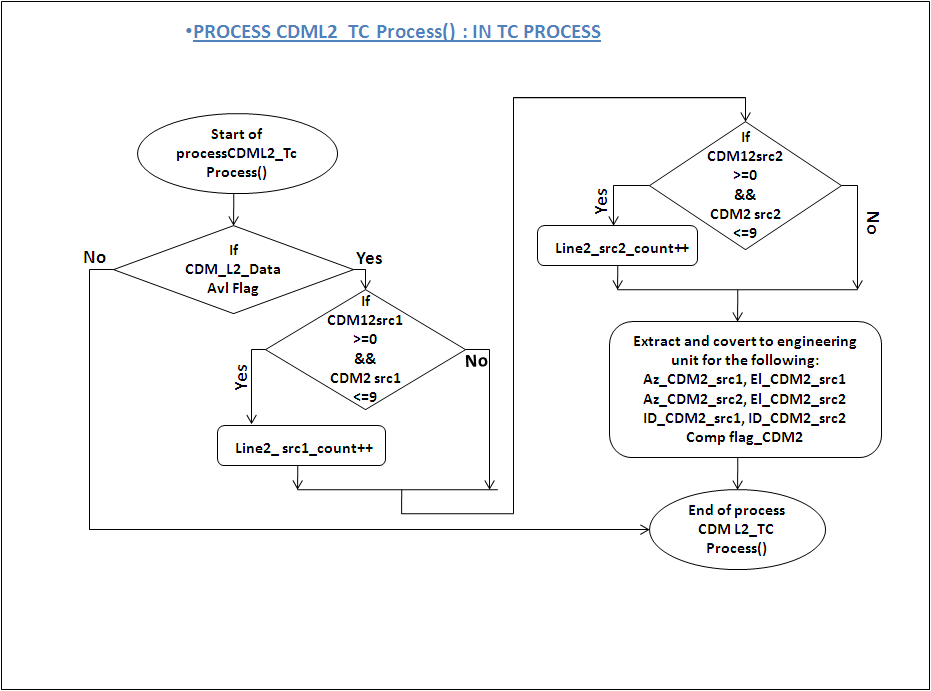
\includegraphics[width=\linewidth]{./FlowCharts/PngFlowCharts/TCP9.png}
	%\caption{Five Chain Configuration of Telecommand}
	%\label{FIG:FiveChConfig}
\end{figure}

\subsection{EDAU flow charts}
\begin{figure}[H]
	\centering
	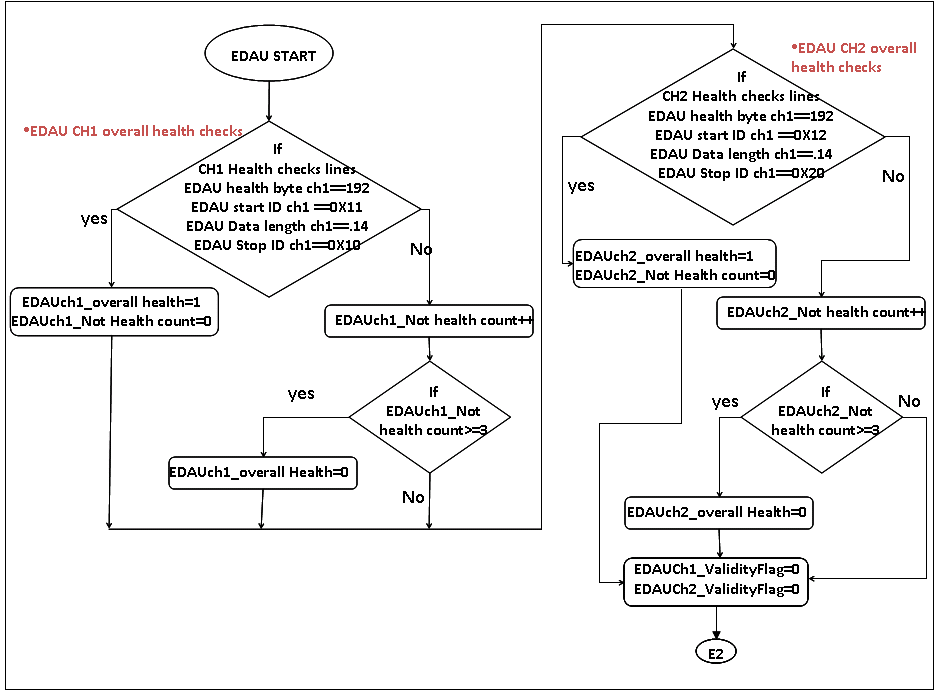
\includegraphics[width=\linewidth]{./FlowCharts/PngFlowCharts/EDAU1.png}
	%\caption{Five Chain Configuration of Telecommand}
	%\label{FIG:FiveChConfig}
\end{figure}

\begin{figure}[H]
	\centering
	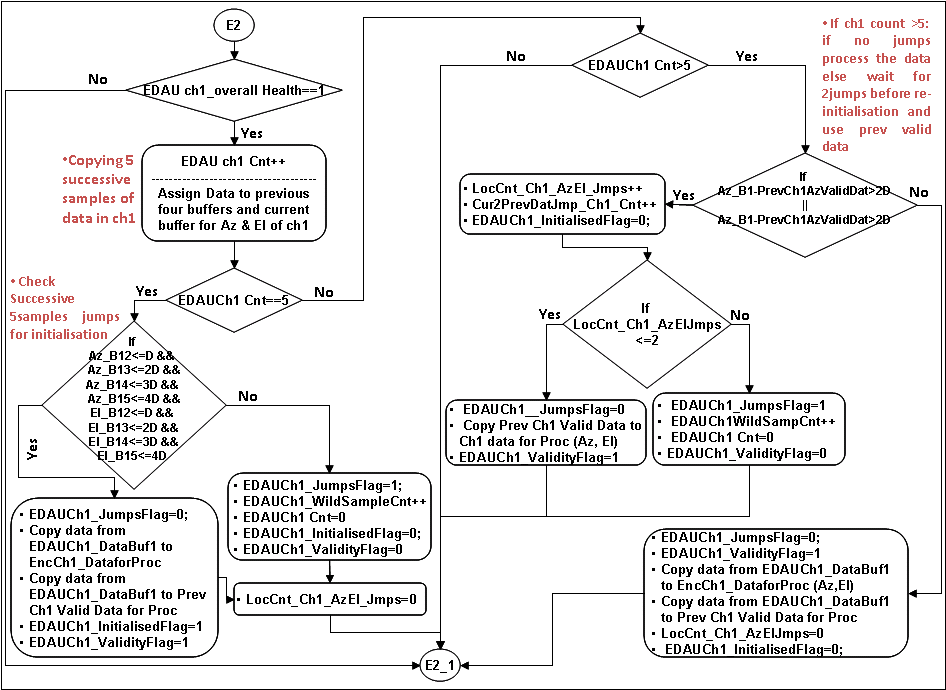
\includegraphics[width=\linewidth]{./FlowCharts/PngFlowCharts/EDAU2.png}
	%\caption{Five Chain Configuration of Telecommand}
	%\label{FIG:FiveChConfig}
\end{figure}

\begin{figure}[H]
	\centering
	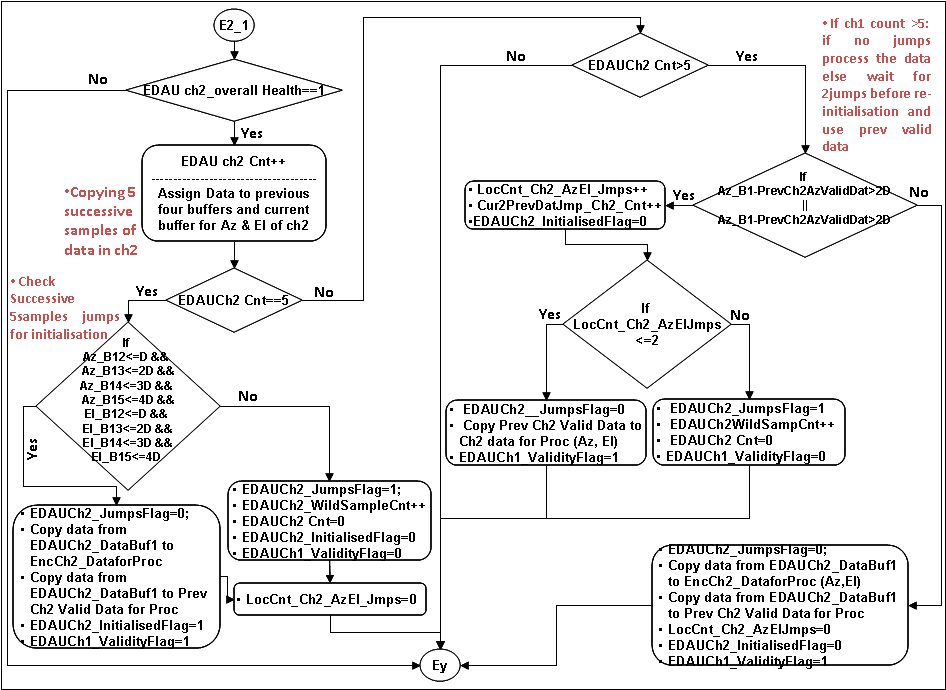
\includegraphics[width=\linewidth]{./FlowCharts/PngFlowCharts/EDAU3.png}
	%\caption{Five Chain Configuration of Telecommand}
	%\label{FIG:FiveChConfig}
\end{figure}

\begin{figure}[H]
	\centering
	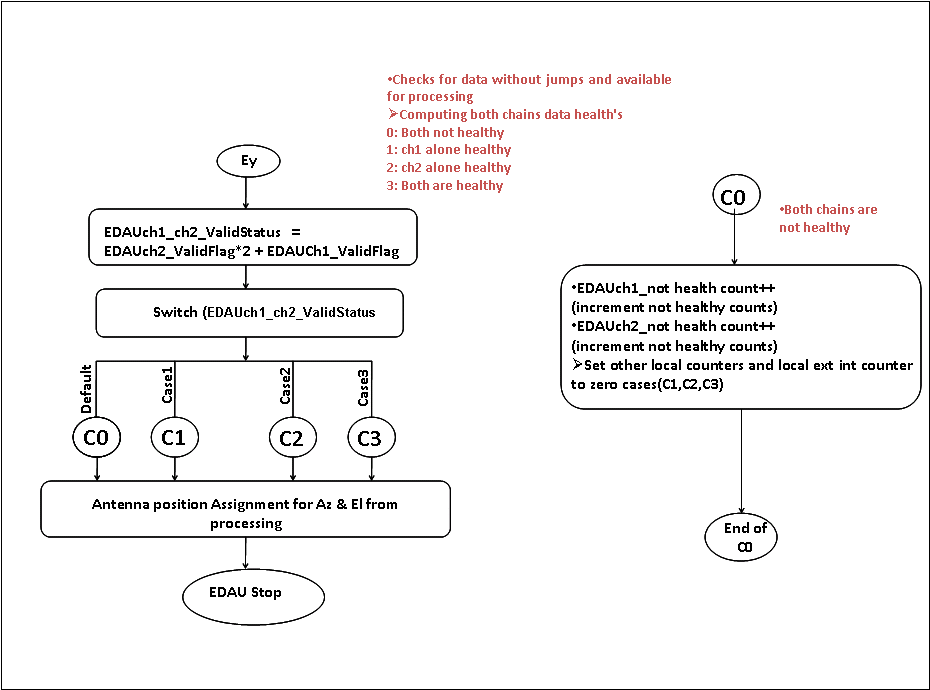
\includegraphics[width=\linewidth]{./FlowCharts/PngFlowCharts/EDAU5.png}
	%\caption{Five Chain Configuration of Telecommand}
	%\label{FIG:FiveChConfig}
\end{figure}


\begin{figure}[H]
	\centering
	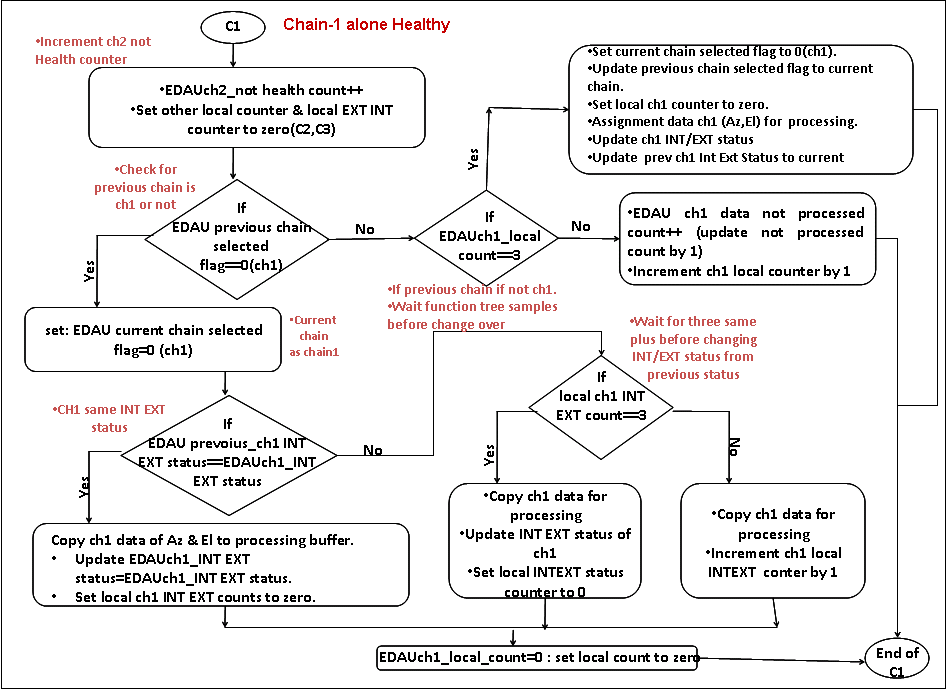
\includegraphics[width=\linewidth]{./FlowCharts/PngFlowCharts/EDAU6.png}
	%\caption{Five Chain Configuration of Telecommand}
	%\label{FIG:FiveChConfig}
\end{figure}


\begin{figure}[H]
	\centering
	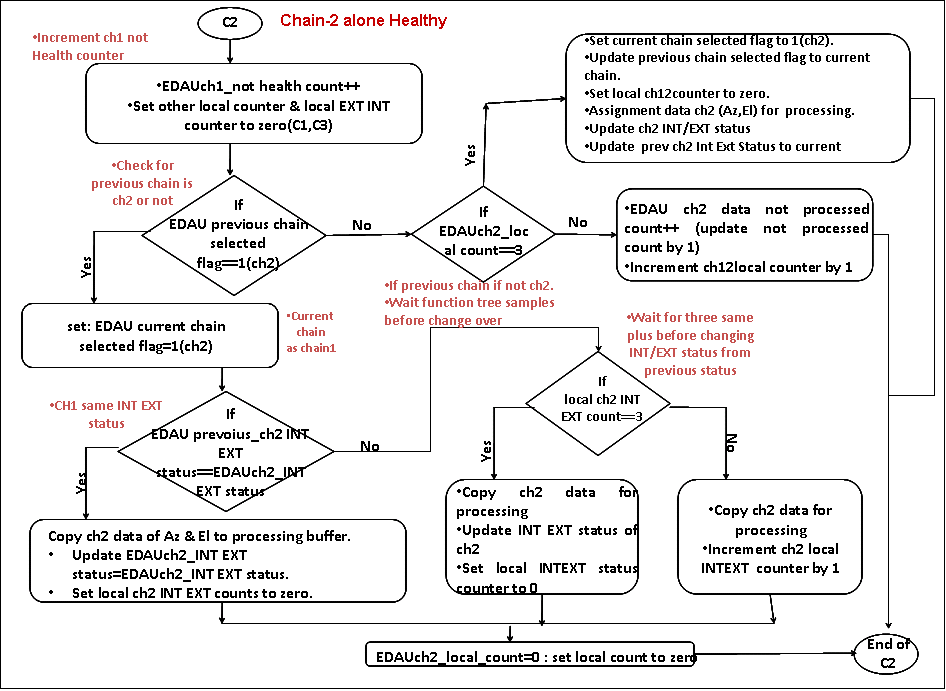
\includegraphics[width=\linewidth]{./FlowCharts/PngFlowCharts/EDAU7.png}
	%\caption{Five Chain Configuration of Telecommand}
	%\label{FIG:FiveChConfig}
\end{figure}


\begin{figure}[H]
	\centering
	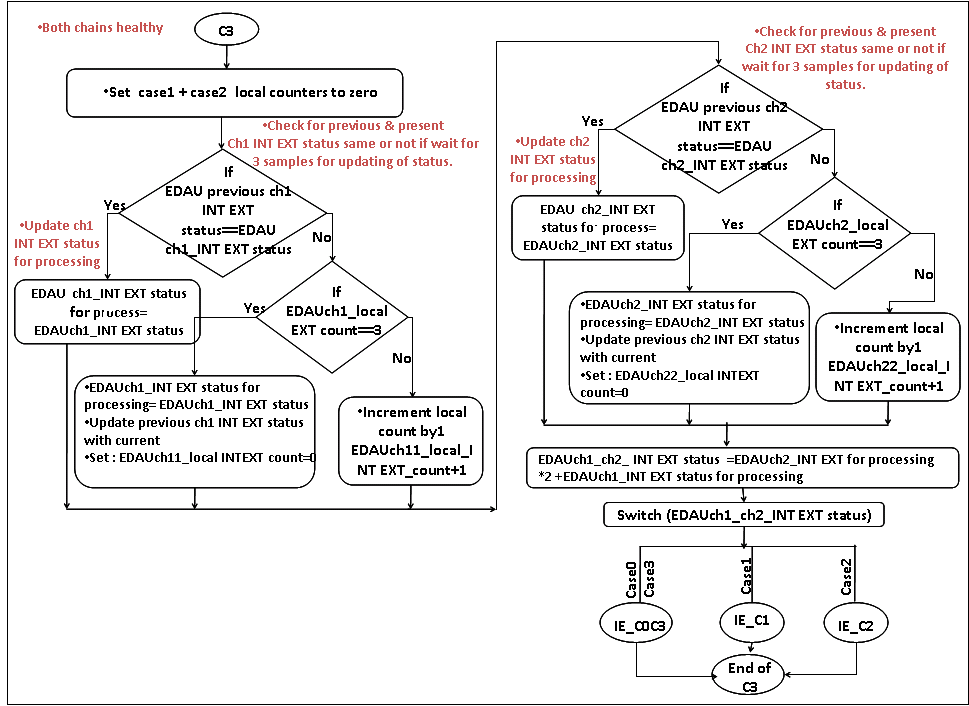
\includegraphics[width=\linewidth]{./FlowCharts/PngFlowCharts/EDAU8.png}
	%\caption{Five Chain Configuration of Telecommand}
	%\label{FIG:FiveChConfig}
\end{figure}


\begin{figure}[H]
	\centering
	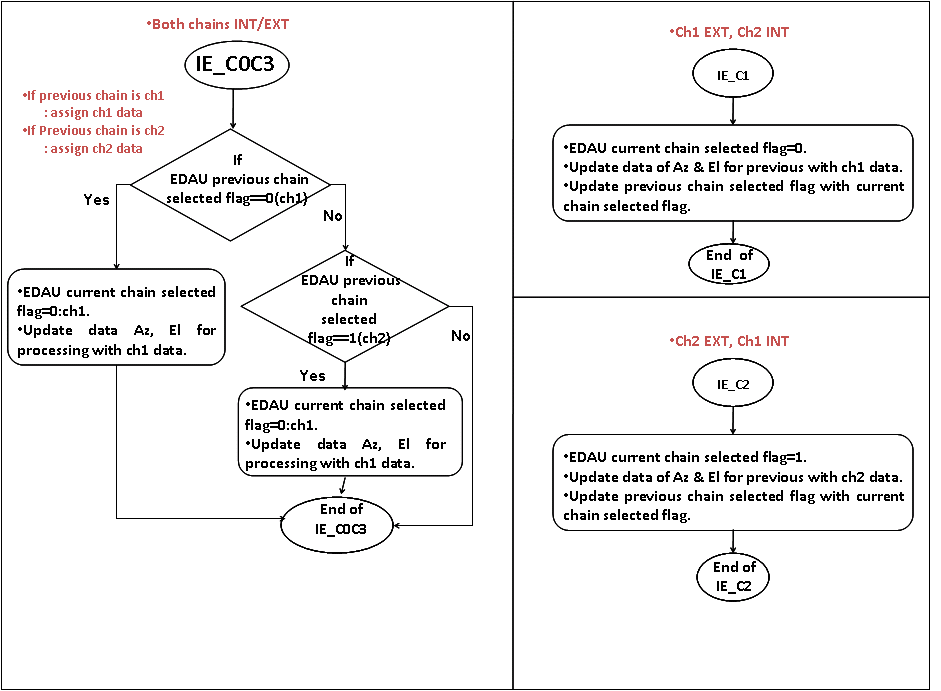
\includegraphics[width=\linewidth]{./FlowCharts/PngFlowCharts/EDAU9.png}
	%\caption{Five Chain Configuration of Telecommand}
	%\label{FIG:FiveChConfig}
\end{figure}




% *************** TC Process Flow charts *******
\section{Analog data input and output}
\subsection{Analog output}
\begin{figure}[H]
	\centering
	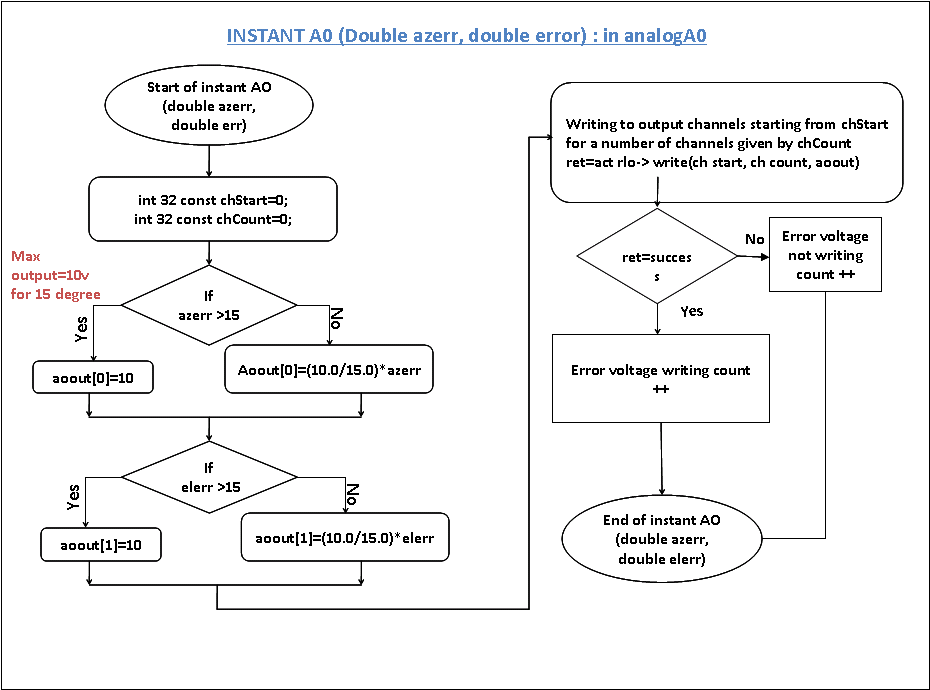
\includegraphics[width=\linewidth]{./FlowCharts/PngFlowCharts/TCP10.png}
\end{figure}
\subsection{Analog input}
\begin{figure}[H]
	\centering
	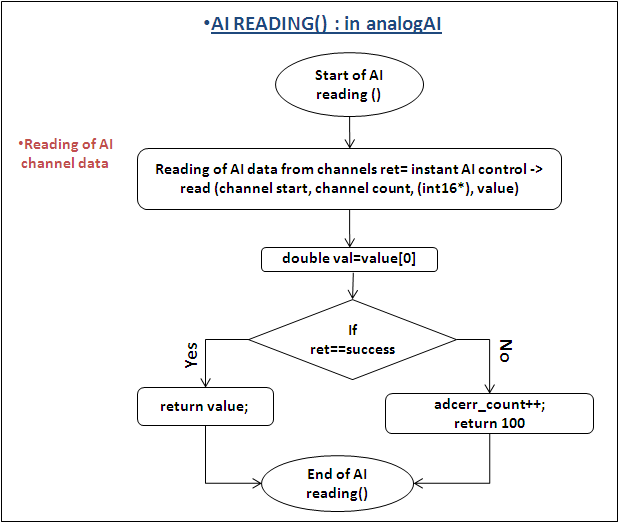
\includegraphics[width=\linewidth]{./FlowCharts/PngFlowCharts/AnalogInput.png}
\end{figure}
\section{Flow charts for concurrent data flow}
\subsection{EDAU serial data reception}
\begin{figure}[H]
	\centering
	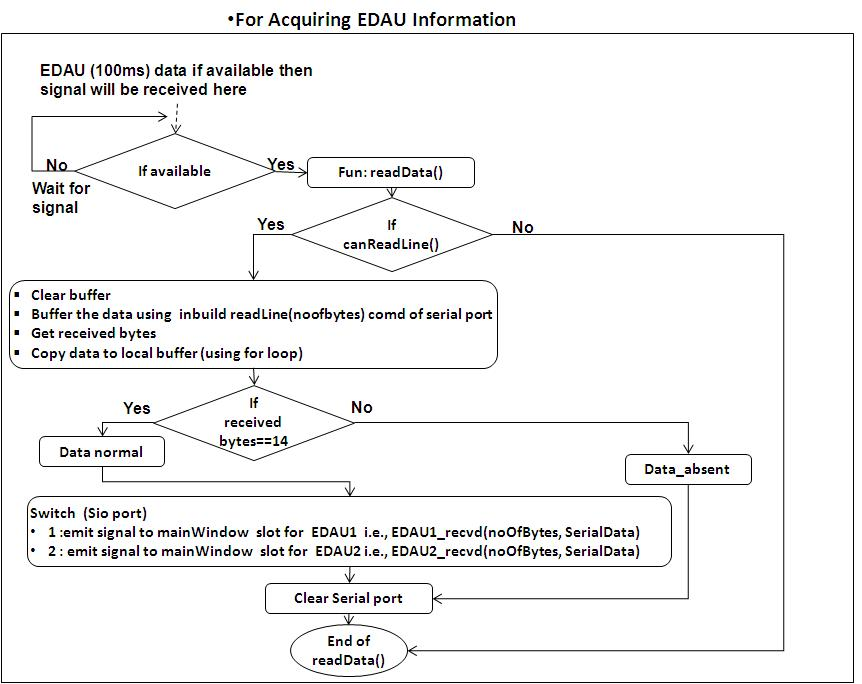
\includegraphics[width=\linewidth]{./FlowCharts/PngFlowCharts/SG1_EDAU.png}
	%\caption{Five Chain Configuration of Telecommand}
	%\label{FIG:FiveChConfig}
\end{figure}
\subsection{CDT serial data reception}
\begin{figure}[H]
	\centering
	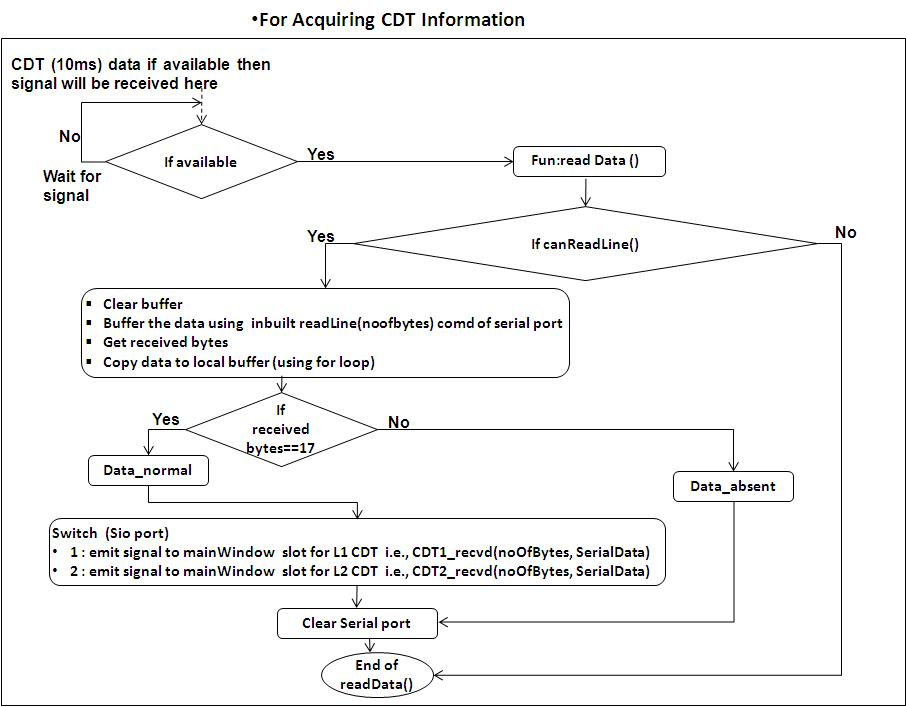
\includegraphics[width=\linewidth]{./FlowCharts/PngFlowCharts/SG2_CDT.png}
	%\caption{Five Chain Configuration of Telecommand}
	%\label{FIG:FiveChConfig}
\end{figure}
\subsection{CDM network reception}
\begin{figure}[H]
	\centering
	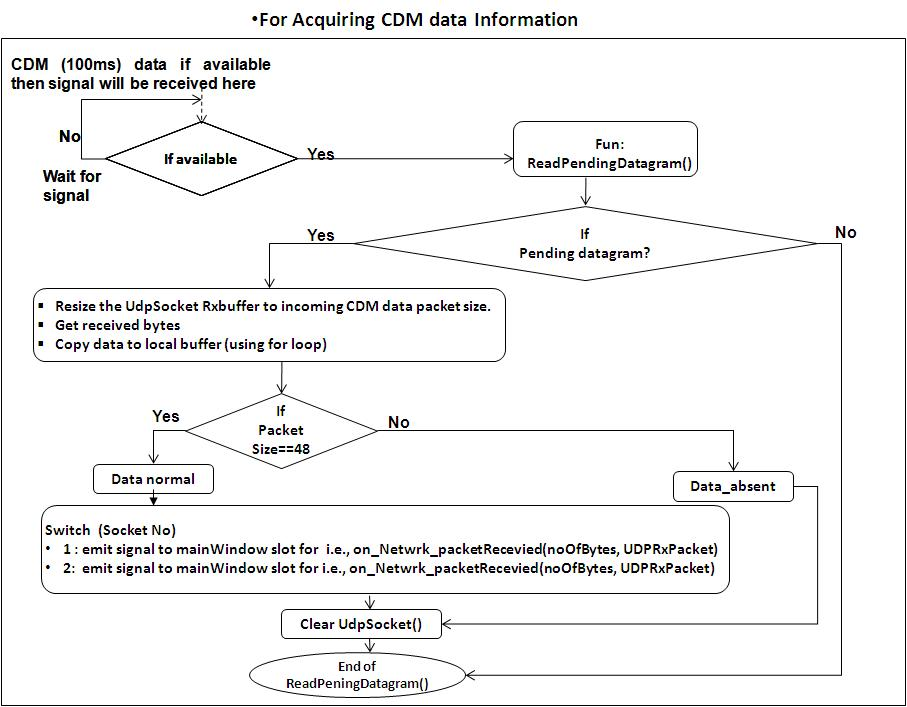
\includegraphics[width=\linewidth]{./FlowCharts/PngFlowCharts/SG3_CDM.png}
	%\caption{Five Chain Configuration of Telecommand}
	%\label{FIG:FiveChConfig}
\end{figure}
\subsection{DI parallel interrupt}
\begin{figure}[H]
	\centering
	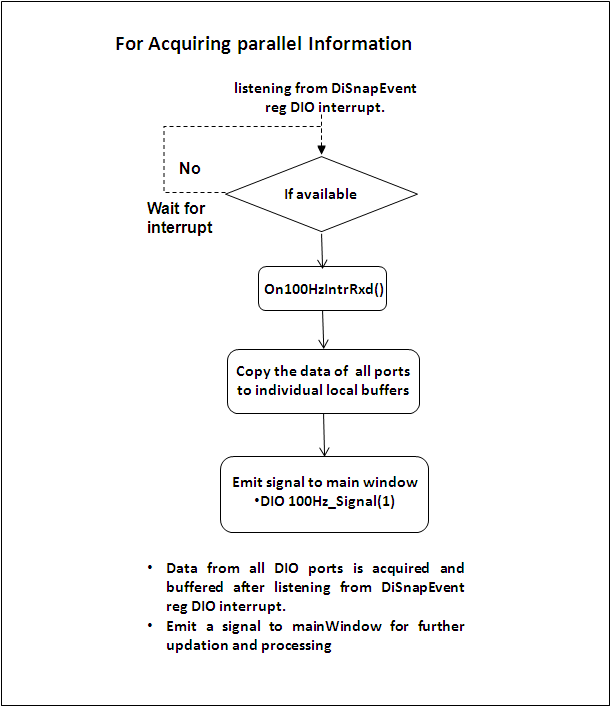
\includegraphics[width=\linewidth]{./FlowCharts/PngFlowCharts/SG4_DIO.png}
	%\caption{Five Chain Configuration of Telecommand}
	%\label{FIG:FiveChConfig}
\end{figure}